% Paty projekt pro predmet ITY
% Autor: Klara Necasova
% Datum: 9.5.2015
\documentclass[pdf]{beamer}
\mode<presentation>{
   \usetheme{CambridgeUS}
   \setbeamercovered{transparent}
}

\usepackage[czech]{babel}
\usepackage[utf8]{inputenc}
\usepackage{graphics}
\usepackage{graphicx}
\usepackage{picture}
\usepackage{eurosym}
\usepackage{multirow}
\newcommand{\myuv}[1]{\quotedblbase #1\textquotedblleft}
 
\title{Tiergarten Sch\"{o}nbrunn}
\subtitle{Zoologická zahrada ve Vídni}
\author{Klára Nečasová}
\institute[FIT VUT]{Fakulta informačních technologií\\Vysoké učení technické v~Brně}
\date{\today}

\begin{document}

% uvodni slide
\begin{frame}
    \titlepage
\end{frame}

 %2. slide
\begin{frame}
\frametitle{Historie}
\begin{itemize}
\item{\textcolor{red}{1752} založena jako zvěřinec císařem Františkem\,I. Štěpánem Lotrinským}
\item{\textcolor{red}{1779} Josef\,II. zpřístupnil zvěřinec bezplatně veřejnosti}
\item{\textcolor{red}{1906} poprvé v~historii se slonu africkému chovanému v~zajetí narodilo mládě}
\item{\textcolor{red}{1921} přešel zvěřinec do majetku republiky}
\item{\textcolor{red}{1997} zapsána na seznam památek UNESCO}
\end{itemize}
\end{frame}

% 3. slide
\begin{frame}
\frametitle{Zajímavosti}
\begin{itemize}
\item{\textcolor{red}{Jihoamerický pavilon}\,--\,lamy, kapybary, tapíři, mravenečníci}
\item{\textcolor{red}{ORANG.erie}\,--\,nový domov vídeňských orangutanů }
\item{\textcolor{red}{Země Františka Josefa}\,--\,pavilon pro lední medvědy, poprvé lze medvědy pozorovat i~při potápění}
\item{\textcolor{red}{Pavilon Aqua Terra}\,--\,terarijní a~akvarijní část je spojena akrylátovým tunelem}
\item{\textcolor{red}{Tropický pavilon} má dvě části}
\setbeamertemplate{itemize items}[triangle]
\begin{itemize}
\item{bažiny a~rýžová pole}
\item{borneovské pralesy (třicetimetrové stromy)}
\end{itemize}
\end{itemize}
\end{frame}

 % 4. slide
\begin{frame}
\frametitle{Zajímavosti}
\begin{itemize}
\item{\textcolor{red}{2007} narodilo se první mládě pandy zplozené přirozenou cestou v~zoologické zahradě}
\item{\textcolor{red}{2010} a~\textcolor{red}{2013} narodilo se druhé a~třetí pandí mládě}
\item{každá panda patří Číně, ať se o~ni stará kdokoliv}
\item{chován medvídek koala, k~vidění v~ZOO jen ojediněle}
\item{krmení zvířat několikrát denně dle rozpisu}
\item{\textcolor{red}{2010} otevřena nová naučná stezka}
\end{itemize}
\centering
  \begin{columns}
  \qquad
   \begin{column}{0.5\textwidth}
   \scalebox{0.1}{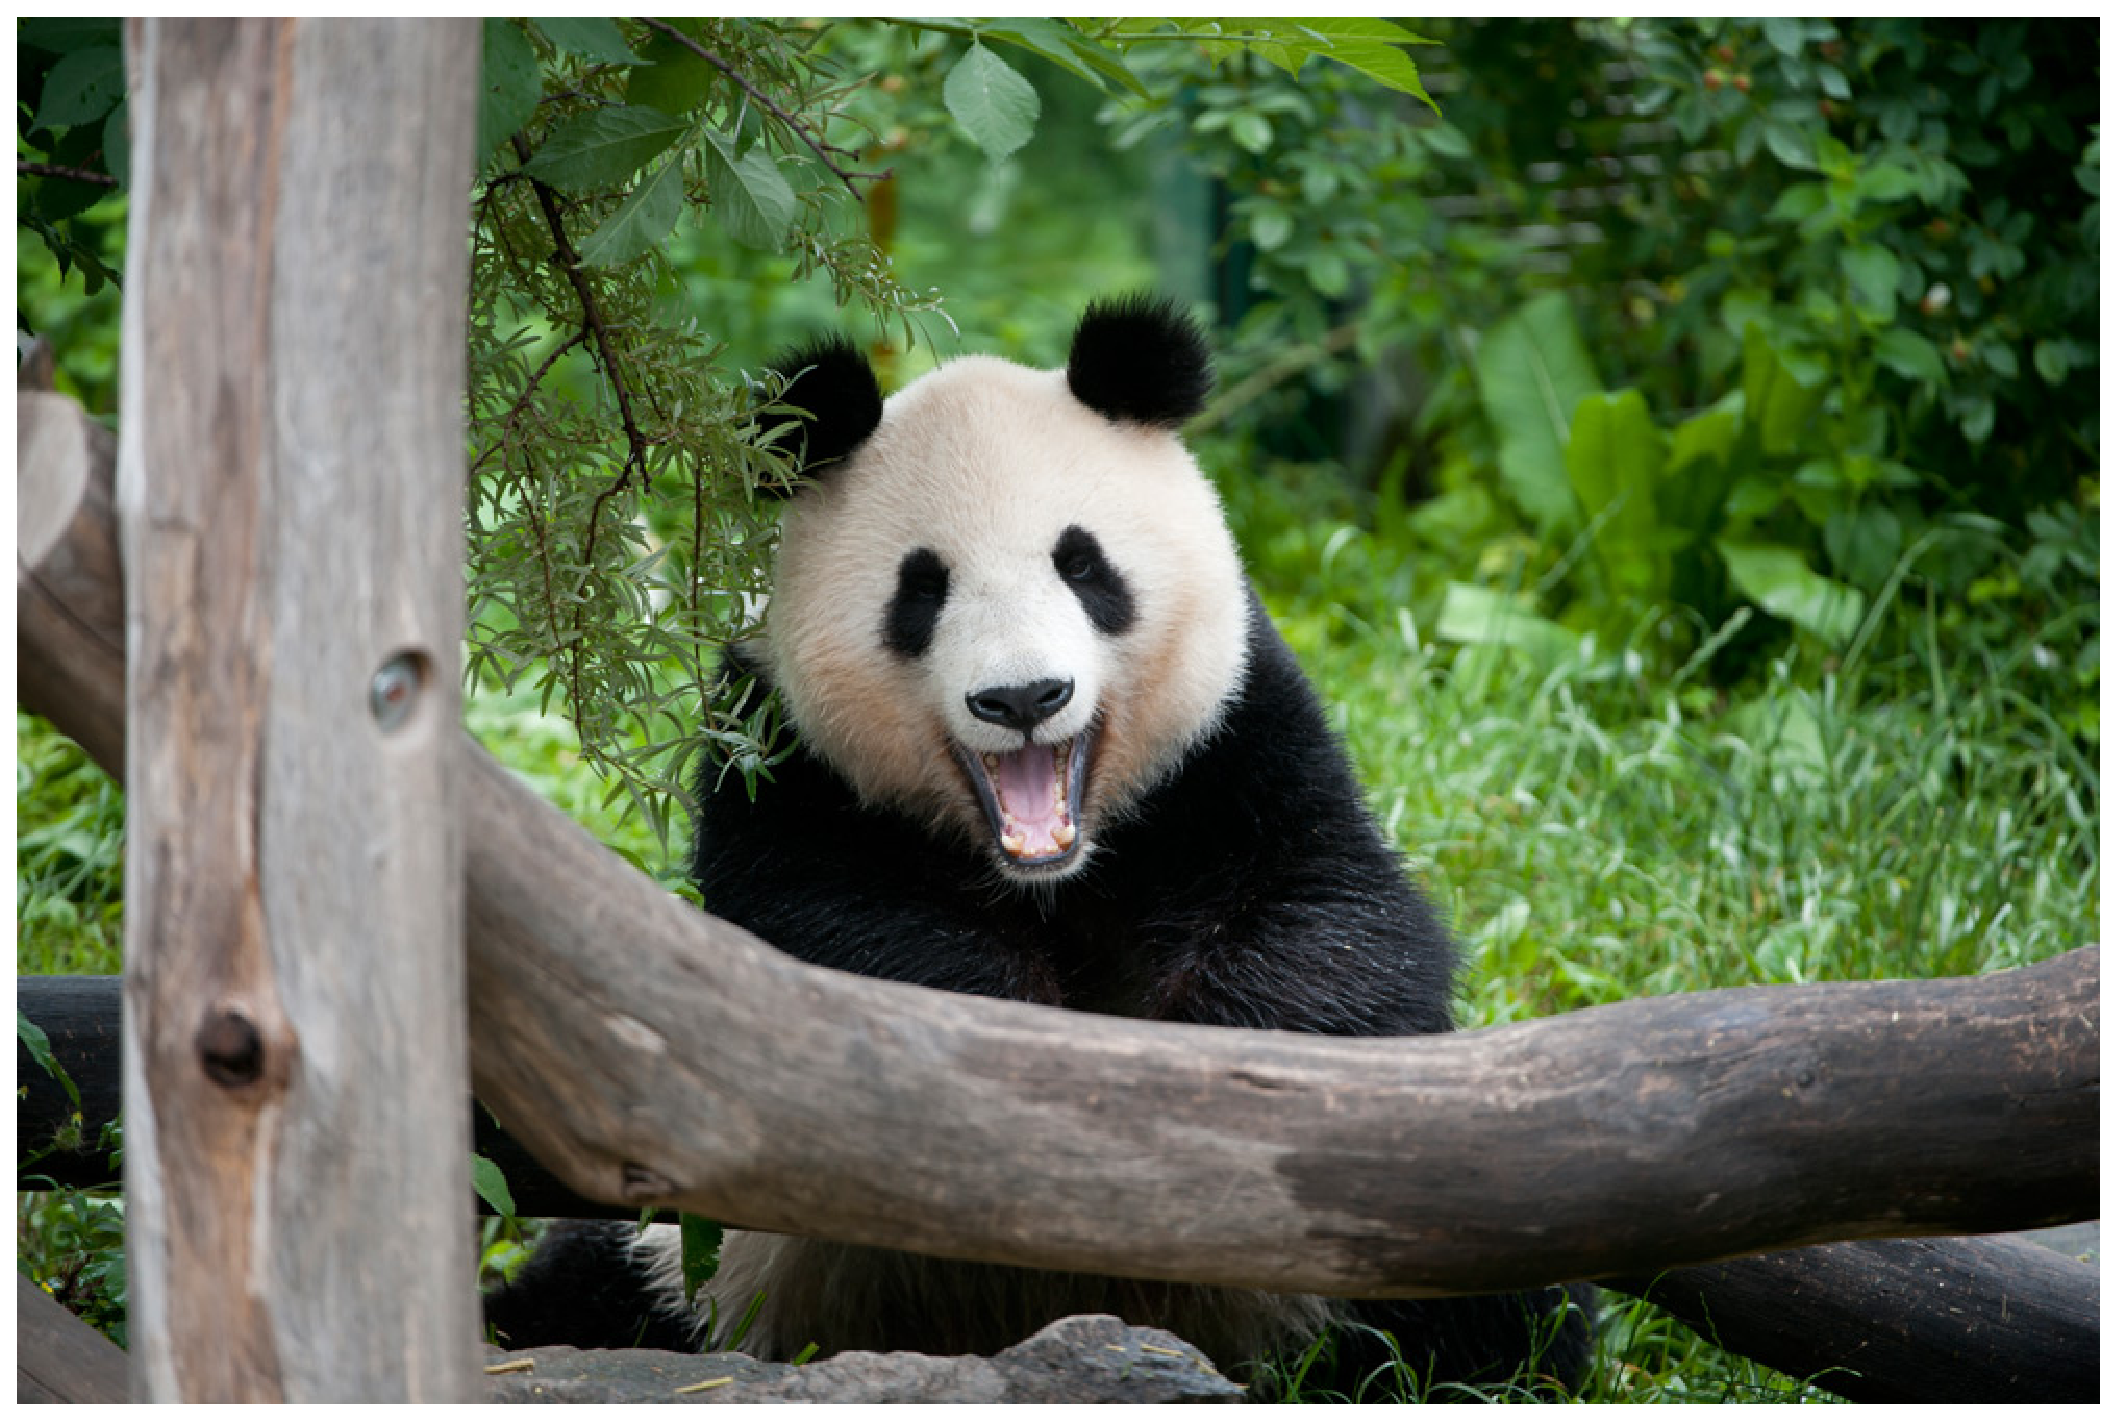
\includegraphics{panda.eps}}
  \end{column}
  \end{columns}
\end{frame}

 % 5. slide
\begin{frame}
\frametitle{Otevírací doba a~vstupné}
\begin{itemize}
\item{otevřeno denně od 9:00 do 16:30 (18:30)}
 \setbeamertemplate{itemize items}[triangle]
\begin{itemize}
\item{zavírací hodina podle ročního období}
\end{itemize}
\setbeamertemplate{itemize items}[ball]
\item{365 dnů v~roce (i~o~svátcích)}
\item{uzavření pokladny a~poslední vstup je půl hodinu před ukončením návštěvní doby}
\begin{table}[h]
\begin{center}
\catcode`\-=12
\begin{tabular}{|c|c|c|}\hline
& Za osobu & Skupiny od 10 osob\\ \hline
Dospělí & \euro\,16,50 & \euro\,14,50\\ \hline
Děti a~mládež & \euro\,8,00 & \euro\,7,00\\ \hline
Osoby se zdravotním  & \multirow{2}{*}{\euro\,8,00} & \multirow{2}{*}{\euro\,7,00}\\ 
postižením (od 50\,\%) & & \\ \hline
Děti do 6 let & zdarma & zdarma\\ \hline
\end{tabular}
\end{center}
\end{table}
\end{itemize}
\end{frame}

% 6. slide
\begin{frame}
\frametitle{Dostupnost dopravními prostředky}
\begin{itemize}
\item{veřejné dopravní prostředky}
\setbeamertemplate{itemize items}[triangle]
\begin{itemize}
\item{metro: linka U4, stanice Hietzing}
\item{tramvaj: 10, 58, 60}
\item{autobus: 10A, 51A, 56A, 56B, 58A}
\end{itemize}
\setbeamertemplate{itemize items}[ball]
\item{automobil}
\setbeamertemplate{itemize items}[triangle]
\begin{itemize}
\item{adresa do navigace\\Seckendorff-Gudent-Weg\\1130 Wien}
\item{parkování ve dvou zařízeních Park \& Ride vzdálených pár stanic metrem od zoologické zahrady }
\item{cestu na parkoviště ukazují informační tabule}
\end{itemize}
\end{itemize}
\end{frame}

% 7. slide
\begin{frame}
\frametitle{Jídlo a~pití}
\begin{itemize}
\item{Tyrolská zahrada}
\setbeamertemplate{itemize items}[triangle]
\begin{itemize}
\item{tyrolská kuchyně, v~létě také grilované speciality}
\end{itemize}
\setbeamertemplate{itemize items}[ball]
\item{Císařský pavilon}
\setbeamertemplate{itemize items}[triangle]
\begin{itemize}
\item{mezinárodní speciality}
\item{možnost pozorování například plameňáků, zeber nebo pand velkých přímo z~terasy}
\end{itemize}
\setbeamertemplate{itemize items}[ball]
\item{Kavárna Atelier Nonja}
\setbeamertemplate{itemize items}[triangle]
\begin{itemize}
\item{kavárenská restaurace s~terasou a~dětským hřištěm}
\item{velký výběr čajů}
\end{itemize}
\setbeamertemplate{itemize items}[ball]
\item{Pivní zahrada}
\setbeamertemplate{itemize items}[triangle]
\begin{itemize}
\item{grilované speciality, křupavé saláty}
\end{itemize}
\end{itemize}
\end{frame}

% 8. slide
\begin{frame}
\frametitle{Zdroje}
\begin{itemize}
\item{oficiální stránky Tiergarten Sch\"{o}nbrunn \\ 
\emph{https://www.zoovienna.at/cs/zoo-a-navstevniku/informace-pro-navstevniky/}}
\item{oficiální stránky města Vídeň \\
\emph{http://www.wien.info/cs/sightseeing/sights/imperial/schoenbrunn-zoo}}
\end{itemize}
\end{frame}

% 9. slide
\begin{frame}
\begin{center}
\Huge{\textcolor{red}{Děkuji za pozornost!}}
\end{center}
\end{frame}

\end{document} 